\section*{M-O Software and External Devices [SSPL Template]}
\label{sec:annex-SSPL}
% In this section briefly describe the software and hardware of the robot

\setlength\intextsep{0pt}
\begin{wrapfigure}[10]{r}{0.3\textwidth}
	\centering
	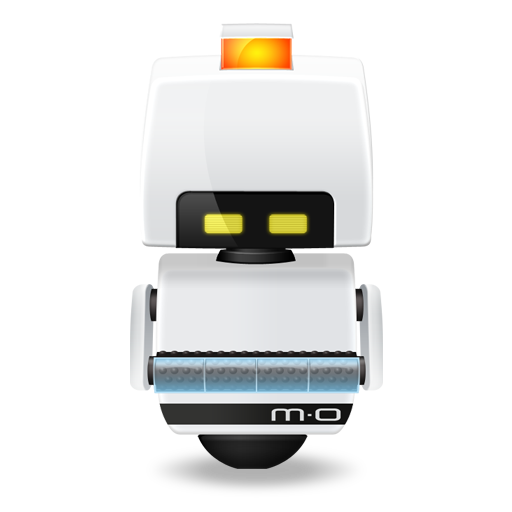
\includegraphics[width=0.4\textwidth]{images/m-o.png}
	\caption{Robot M-O}
	\label{fig:m-o}
\end{wrapfigure}

We use a standard \textit{Buy'N Large} M-O robot unit. To differntiate our unit, an orange marker has been added on its top.

\section*{Robot's Software Description}
% Please describe in this section the software you are using to control your robot. Consider the following example:

\textit{For our robot we are using the following software:}

\begin{itemize}
	\item Platform: \BnL Operating System
	\item Face recognition: None. Not designed for human interaction.
	\item Speech generation: None. Not designed for human interaction.
	\item Object recognition: \BnL Dirt Detector Algorithm (See previous sections).
	\item Mop unit: \BnL automatic controller \cite{bnl2}.
\end{itemize}

\section*{External Devices}
% Please describe in this section the external devices used by your robot. Consider the following example:

\textit{M-O robot relies on the following external hardware:}

\begin{itemize}
	\item \BnL Mother-ship
	\item \BnL Data Cluster
	\item $3 \times$ \BnL Ultra-Power laptops.
\end{itemize}

\section*{Cloud Services}
% Please describe in this section the Cloud Services and online software used by your robot. Consider the following example:

\textit{M-O connects the following cloud services:}
\begin{itemize}
	\item Localization and mapping: \BnL Geolocalization system \cite{bnl3}.
	\item Navigation: \BnL Navigator
	\item Speech recognition: \BnL All-purpose recognizer \cite{bnl1}.
\end{itemize}